\documentclass[UTF-8]{ctexart}

\usepackage{amsmath}
\usepackage{enumerate}
\newtheorem{definition}{Definition}[section]
\newtheorem{axiom}{公理}[section]
\newtheorem{theorem}{Theorem}[section]
\newtheorem{lemma}{Lemma}
\newtheorem{proof}{Proof}[section]

\usepackage{graphicx} %插入图片的宏包
\usepackage{float} %设置图片浮动位置的宏包
\usepackage{subfigure} %插入多图时用子图显示的宏包

% 开始文档
\begin{document}

% 创建标题页的内容
\title {数学学习笔记} \author{cpd} \date{2023/11/12}
% 生成标题
\maketitle

% 设置页码格式是罗马数字
\pagenumbering{roman}
% 生成目录
\tableofcontents
% 插入新页
\newpage
% 设置页码格式是阿拉伯数字
\pagenumbering{arabic}

\section{实分析}
\subsection{公理}

\begin{axiom}
\label{axiom1}
0 是一个自然数.
\end{axiom}

\begin{axiom}
\label{axiom2}
若n 是自然数, 则n++ 也是自然数.
\end{axiom}

\begin{axiom}
    \label{axiom3}
    0不是任何自然数的后继,即对于每个自然数n,都有$n++ \ne 0$
\end{axiom}
\begin{axiom}
    \label{axiom4}
不同的自然数必定有不同的后继者;也就是说,若n,m是自然数且$n \ne m$,则$n++\ne m++$.等
价地说,若n++=m++,则必有n=m.
\end{axiom}

\begin{axiom}
    \label{axiom5}
(数学归纳原理) 设$P(n)$是关于自然数的一个性质.假设$P(0)$是真的,并且只要$P(n)$为
真可以推导出$P(n++)$为真,那么对于每个自然数$n$,$P(n)$都是真的.
\end{axiom}
\subsection{定义}

\begin{definition}
定义1是数0++,2数数(0++)++,3是数((0++)++)++,等等.
\end{definition}

\begin{definition}
存在一个数系$N$,称其元素为自然数,公理\ref{axiom1} \~{} \ref{axiom5} 对此数系成立.
\end{definition}

\begin{definition}
(自然数的加法) 设m是自然数.我们定义$0+m:=m$.现在归纳假定已定义好如何使m加上n,那
么把m加于n++定义为$(n++)+m:=(n+m)++$.
\end{definition}

\begin{definition}
(正自然数) 一个自然数叫做正的,当且仅当它不等于0.
\end{definition}

\begin{definition}
  (自然数的排序) 设n和m是自然数.我们说n大于等于m,记作$n \geq m$或$m \leq n$,当且
  仅当对于某自然数a,成立n=m+a.我们说n严格大于m,记作$n>m$或$m<n$,当且仅当$n\geq m
  $并且$n \ne m$.
\end{definition}

\begin{definition}


(自然数的乘法) 设m是自然数.我们定义$0 \times  m:=0$.设已定义了如何把n乘到m上,那么归纳地,我们定义把n++乘到m上是(n++) $ \times $ m:=(n $ \times $ m)+m.
\end{definition}

\subsection{定理}

\begin{theorem}
设对于每个自然数n,都有某个函数$f_n:N->N$把自然数映成自然数.设c是一个自然数,那么
可以对于每个自然数n指定唯一一个自然数$a_n$,使得$a_0=c$且$a_{n++}=f_n(a_n)$.
\end{theorem}

\begin{theorem}
  对于任何自然数n,$n+0=n$.
\end{theorem}

\begin{theorem}
  对于任何自然数n和m,$n+(m++)=(n+m)++$.
\end{theorem}

\begin{theorem}
(加法是交换的)  对于任何自然数n和m,n+m=m+n.
\end{theorem}

\begin{theorem}
(加法是结合的)  对于任何自然数a,b,c,$(a+b)+c=a+(b+c)$.
\end{theorem}

\begin{theorem}
(消去律)  设a,b,c是自然数,满足a+b=a+c,我们有b=c.
\end{theorem}

\begin{theorem}
若a是正的而b是自然数,则a+b是正的.
\end{theorem}

\begin{theorem}
如果a和b是自然数,满足a+b=0,那么a=0且b=0.
\end{theorem}

\begin{theorem}
设a是正数,那么恰存在一个自然数b,使得b++=a.
\end{theorem}

\begin{theorem}
  (自然数的序的基本性质) 设a,b,c是自然数.那么
\begin{enumerate}[(a)]
\item (序是自反的)$a\geq a$
\item (序是传递的)若$a \geq b$且$b \geq c$,那么$a \geq c$.
\item (序是反对称的)若$a \geq b$且$b \geq a$,那么$a \eq b$.
\item (加法保序)$a \geq b$当且仅当$a+c \geq b+c$
\item $a < b $当且仅当$a++ \leq b$
\item $a < b $当且仅当对于某正数d,$b=a+d$
\end{enumerate}
\end{theorem}

\begin{theorem}
  (自然数的序的三歧性)设a和
  b是自然数,那么下述三命题中恰有一个是真的:
  $$a<b,a=b,a>b$$
\end{theorem}

\begin{theorem}
(强归纳法原理)设$m_0$是一个自然数,而$P(m)$是一个依赖于任意自然数m的性质.设对于每
个$m \geq m_0$都有下述蕴含关系:如果$P(m^')$对于一切满足$m_0 \leq m^{'}  < m$的自然
数$m^'$都成立,那么$P(m
)$也成立(特别地,这意味着$P(m_0)$成立,因为在$m=m_0$的情况下,假定的条件$P(m^')$是
空的),那么,我们可以断定$P(m)$对于一切自然数$m \geq m_0$都成立.
\end{theorem}

\newpage
\section{微积分}
\subsection{多重积分}
\subsubsection{定义}
多重积分(英语:Multiple integral)是定积分的一类,它将定积分扩展到多元函数(多
变量的函数),例如求$f(x,y)$或者$f(x,y,z)$类型的多元函数的积分.

正如单变量的正函数的定积分代表函数图像和x轴之间区域的面积一样,正的双变量函数的
双重积分代表函数所定义的曲面和包含函数定义域的平面之间所夹的区域的体积。(注意同
样的体积也可以通过三变量常函数 $f(x,y,z)=1$ 在上述曲面和平面之间的区域中的三重积分得到。若有更多变量,则多元函数的多重积分给出超体积。

n元函数$f(x_1,x_2,...,x_n)$在定义域D上的多重积分通常用嵌套的积分号按照演算的逆序
标识(最左边的积分号最后计算),后面跟着被积函数和正常次序的积分变量(最右边的变
量最后使用)。积分域或者对每个积分变量在每个积分号下标识,或者用一个变量标在最右
边的积分号下:

$\int\ldots\int_{\mathbf{D}} f(x_{1},x_{2},\ldots,x_{n}) \mathrm{d}x_{1}\ldots\mathrm{d}x_{n}$

因为不可能计算多于一个自变量的函数的不定积分,“不定”多重积分是不存在的。因此所有多重积分都是“定”积分。

通常在坐标系中,多重积分都利用嵌套的累次积分计算。而累次积分为了简便可记为:

$\int_{\varphi_{1}}^{\psi_{1}}\mathrm{d}x_{1}\int_{\varphi_{1}(x_{1})}^{\psi_{2}(x_{1})}\mathrm{d}x_{2}\ldots\int_{\varphi_{n}(x_{1},x_{2},\ldots,x_{n-1})}^{\psi_{n}(x_{1},x_{2},\ldots,x_{n-1})}f(x_{1},x_{2},\ldots,x_{n})\mathrm{d}x_{n}$

其中积分域为:

$D=\{(x_1,x_2,\ldots,x_n)|\varphi_1\leq
x_1\leq\dot{\varphi}_1,\varphi_2(x_1)\leq
x_2\leq\dot{\varphi}_2(x_1),\ldots,\varphi_n(x_1,x_2,\ldots,x_{n-1})\leq
x_n\leq\psi_n(x_1,x_2,\ldots,x_{n-1})\}$
注意的是,该式一般情况下并不表示多个定积分的积,在实际计算中从最右侧积分变量开始积分,其结果会作为外一层积分的被积函数。

\subsubsection{积分方法}
多重积分问题的解决在多数情况下依赖于将多重积分转化为一系列单变量积分,而其中每个单变量积分都是直接可解的。

\paragraph{直接检验}
有时可以直接获得积分的结果,而无需任何直接计算。

\paragraph{常数}
在常函数的情况中,结果很直接:只要将常函数c乘以测度就可以了。如果c = 1,而且是在$R^2$$的子集中积分,则乘积就是区域面积,而在$R^3$中,它就是区域的体积。

例如:
$D = \{ (x,y) \in \mathbb{R}^2 \ : \ 2 \le x \le 4 \ ; \ 3 \le y \le 6 \}</math> and <math>f(x,y) = 2$

在D上积分f:
$\int_3^6 \int_2^4 \ 2 \ \mathrm{d}x\, \mathrm{d}y = \mbox{area}(D) \cdot 2 = (2 \cdot 3) \cdot 2 = 12$
\paragraph{利用可能的对称性}
如果定义域存在沿着某条轴的对称性而且函数对于那个变量是奇函数,则积分为0(因为相反的两部分加起来为0)。

对于$R^n$中的函数,只要相关变量对于形成对称的轴是奇变量就可以了。

例一:
给定$f(x,y) = 2 \sin(x)-3y^3+5$以及$T=\left \{ ( x,y) \in \mathbf{R}^2 \ : \ x^2+y^2\le 1 \right \}$为积分区域(半径为1的圆盘,包含边界)。

利用线性性质,积分可以分解为三部分:

$\iint_T (2\sin x - 3y^3 + 5) \, \mathrm{d}x \, \mathrm{d}y = \iint_T 2 \sin x \, \mathrm{d}x \, \mathrm{d}y - \iint_T 3y^3 \, \mathrm{d}x \, \mathrm{d}y + \iint_T 5 \, \mathrm{d}x \, \mathrm{d}y$

$2\sin(x)$ 和 $3y^3$ 都是奇函数,而且显然T对于x和y轴都是对称的;因此唯一有贡献的部分是常函数5,因为其它两个都贡献0.

例二:
考虑函数$f(x,y,z)=x \exp(y^2+z^2)$以及圆心在原点的半径为2的球
$T = \left \{ ( x,y, z) \in \mathbf{R}^3 \ : \ x^2+y^2+z^2 \le 4 \right \}$
该球显然是对于三条轴都对称,但是只要对于x轴积分就可以看出结果是0,因为f对于该变量是奇函数。

\paragraph{简化公式}
简化公式基于简单积分区域来将多重积分转化为单变量积分的序列。它们必须从右至左计算,过程中将其它变量暂时视为常数(和偏导数的计算类似)。

\subparagraph{$R^2$中的常规区域}
此种方法适用于满足下述条件的任何定义域 D:
1. D 投影到 x轴或 y轴任一轴,形成一个有边界的范围, 以 a, b 代表边界值。
2. 通过 a, b 两点并与$\overline {ab}$ 垂直的直线与 D 相交后的两个端点,可以用 2 个函数$\alpha , \beta $.

X轴:将D 对x轴做垂直投影,函數$f: D \longrightarrow \mathbb{R}$是连续函数,并且D可以视为(定义在[a,b]区间上的)α(x)和β(x)之间的区域。则

$\iint_D f(x,y)\ \mathrm{d}x\, \mathrm{d}y = \int_a^b \mathrm{d}x \int_{ \alpha (x)}^{ \beta (x)} f(x,y)\, \mathrm{d}y$

y:
将D 对y轴做垂直投影,函數$f: D \longrightarrow \mathbb{R}$是连续函数,并且D可以视为(定义在[a,b]区间上的)α(y)和β(y)之间的区域。则

$\iint_D f(x,y)\ \mathrm{d}x\, \mathrm{d}y = \int_a^b \mathrm{d}y \int_{ \alpha (y)}^{ \beta (y)} f(x,y)\, \mathrm{d}x$

范例:
考虑区域:$D = \{ (x,y) \ : \ x \ge 0, y \le 1, y \ge x^2 \}$(参看附图)。计算

$\iint_D (x+y) \, \mathrm{d}x \, \mathrm{d}y$

该区域可以沿x或者y轴分解。要采用公式,必须先找到限制''D''的两个函数和定义区间。
这个例子中,这两个函数为:

$\alpha (x) = x^2\,\!</math> 和 <math>\beta (x) = 1\,\!$

而区间为<math>[a,b] = [0,1]\,\!</math>(这里为了直观起见采用沿x轴分解)。

应用简化公式,得到:

$\iint_D (x+y) \, \mathrm{d}x \, \mathrm{d}y = \int_0^1 \mathrm{d}x \int_{x^2}^1 (x+y) \, \mathrm{d}y = \int_0^1 \mathrm{d}x \ \left[xy \ + \ \frac{y^2}{2} \ \right]^1_{x^2}$

(首先,第二个积分将x作为常数)。然后就是用积分的基本技术:

$\int_0^1 \left[xy \ + \ \frac{y^2}{2} \ \right]^1_{x^2} \, \mathrm{d}x = \int_0^1 \left(x + \frac{1}{2} - x^3 - \frac{x^4}{2} \right) \mathrm{d}x = \cdots = \frac{13}{20}$

如果沿着y轴分解,可以计算
$\int_0^1 \mathrm{d}y \int_0^{\sqrt{y}} (x+y) \, \mathrm{d}x$

并得到同样的结果。
\subparagraph{$R^3$中的常规区域}
这些公式可以推广到三重积分:

T是一个可以投影到xy平面的体,它夹在α(x,y)和β(x,y)两个函数之间。那么:

$\iiint_T f(x,y,z) \ \mathrm{d}x\, \mathrm{d}y\, \mathrm{d}z = \iint_D \mathrm{d}x\, \mathrm{d}y \int_{\alpha (x,y)}^{\beta (x,y)} f(x,y,z) \, \mathrm{d}z$

(此定义和其它$R^3$$中的分解类似)。

\subparagraph{变量替换}
积分的极限常常不易交换(区域无法分解或者公式很复杂),这时可以采用变量替换来重写积分,令区域更加简易,从而可以用更简单的公式表达。为此,函数必须变换到新坐标系下。

函数为$f(x, y) = (x-1)^2 +\sqrt y$;

若采用替换$x' = x-1, \ y'= y $则$x = x' + 1, \ y=y' $

可以得到新函数$f_2(x,y) = (x')^2 +\sqrt y$.

对于定义域要进行类似处理,因为原来是采用变换前的变量表达的(本例中的x和y)

微分dx和dy要通过包含被替换的变量对于新变量的偏微分的[[雅可比行列式]]来变换。(譬如,极坐标的微分变换)。

常用的变量替换有三种($R^2$中一种,$R^3$中两种);但是,更普遍的变换可以用同样的原理来发现。

\subparagraph{极坐标}
在$R^2$中,若定义域有某种圆形对称性而函数也有某种特征,则可以采用极坐标变换(参看图中的例子),也就是说将点$P(x,y)$从笛卡尔坐标变换到相应的极坐标中。这使得定义域的形状改变,从而简化运算。

该变换的基本关系如下:

$f(x,y) \rightarrow f(\rho \ \cos \phi,\rho \ \sin \phi )$。

例子1,
函数为$f(x,y) = x + y$

应用该变换得到$f(\rho, \phi) = \rho \cos \phi + \rho \sin \phi = \rho \ (\cos \phi + \sin \phi )$。

例子2,
函数为$f(x,y) = x^2 + y^2$
应用该变换到得$f(\rho, \phi) = \rho^2 (\cos^2 \phi + \sin^2 \phi) = \rho^2\$

这里使用了勾股定理(在简化操作时很有用)。

定义域的变换是根据x和y通过环厚和角度的幅度来限定ρ, φ的区间。

例子3,
区域为$D = x^2 + y^2 \le 4$,圆周半径2;很明显,这个区域所覆盖的角度是整个圆周角,所以φ从0变化到2π,而环半径从0变化到2(内环为0的环形就是圆)。

例子3,
区域为 $D = \{ x^2 + y^2 \le 9, \ x^2 + y^2 \ge 4, \ y \ge 0 \}$,这是在正y半平面中的圆环(参看示意图);注意φ表示平面角而ρ从2变化到3。因此变换出来的区域为矩形:$T = \{ 2 \le \rho \le 3, \ 0 \le \phi \le \pi \}$

该变换的雅可比行列式为:

:<math>\frac{\partial (x,y)}{\partial (\rho, \phi)} =
\begin{vmatrix}
\cos \phi & - \rho \sin \phi \\
\sin \phi & \rho \cos \phi
\end{vmatrix} = \rho</math>

这可以通过将''x'' = ρ cos(φ), ''y'' = ρ sin(φ)代入关于ρ的第一行和关于φ的第二行的偏微分中得到,所以微分''dx dy''变换为ρ ''d''ρ ''d''φ.

一旦函数和区域的变换完成后,可以定义极坐标中的变量变换公式:

:<math>\iint_D f(x,y) \ \mathrm{d}x\, \mathrm{d}y = \iint_T f(\rho \cos \phi, \rho \sin \phi) \rho \, \mathrm{d} \rho\, \mathrm{d} \phi</math>。

注意φ在[0, 2π]区间中有效,而ρ测量长度,因此只能取非负值。

此外,应用变量变换公式的前提是,雅可比行列式的值在变换后的积分变量(如此例中的ρ和φ)组成的有界闭区域(如此例中φ和ρ构成的二维域)上恒不为零。但是在极坐标中当且仅当ρ为零时,才有雅可比行列式为零,故可证明该变量变换公式成立。



<u>例 (2-e)</u>:
:函数为<math>f(x,y) = x\,\!</math>区域和例2-d相同。
:从前面对''D''的分析,我们知道ρ的区间为[2,3],而φ的为[0,π].函数变换为:

::<math>f(x,y) = x \longrightarrow f(\rho,\phi) = \rho \ \cos \phi</math>。

:最后,应用积分公式:

::<math>\iint_D x \, \mathrm{d}x\, \mathrm{d}y = \iint_T \rho \cos \phi \ \rho \, \mathrm{d}\rho\, \mathrm{d}\phi</math>。

:一旦区间给定,就可以得到

::<math>\int_0^{\pi} \int_2^3 \rho^2 \cos \phi \ \mathrm{d} \rho \ \mathrm{d} \phi = \int_0^{\pi} \cos \phi \ \mathrm{d} \phi \left[ \frac{\rho^3}{3} \right]_2^3 = \left[ \sin \phi \right]_0^{\pi} \ \left(9 - \frac{8}{3} \right) = 0</math>。
</blockquote>

==== 柱极坐标 ====
[[File:Cylindrical Coordinates.svg|thumb|190px|柱极坐标。]]
'''R'''<sup>3</sup>中,在有圆形底面的定义域上的积分可以通过变换到[[柱极坐标系]]来完成;函数的变换用如下的关系进行:
<center><math>f(x,y,z) \rightarrow f(\rho \cos \phi, \rho \sin \phi, z)</math> </center>

区域的变换可以从图形中得到,因为底面的形状可能不同,而高遵循初始区域的形状。

<blockquote>
<u>例(3-a)</u>: <br />
:区域为<math>D = \{ x^2 + y^2 \le 9, \ x^2 + y^2 \ge 4, \ 0 \le z \le 5 \}</math>(也即底面为例2-d中的圆环的高度为5的"管道");如果采用变换,可以得到区域<math>T = \{ 2 \le \rho \le 3, \ 0 \le \phi \le \pi, \ 0 \le z \le 5 \}</math>(这是一个底面为例2-d中的矩形而高为5的长方体)。

因为''z''分量没有变化,''dx dy dz''和在极坐标中一样变化:变为''ρ dρ dφ dz''。

最后,变换到柱极坐标的最后公式为:

:<math>\iiint_D f(x,y,z) \, \mathrm{d}x\, \mathrm{d}y\, \mathrm{d}z = \iiint_T f(\rho \cos \phi, \rho \sin \phi, z) \rho \, \mathrm{d}\rho\, \mathrm{d}\phi\, \mathrm{d}z</math>。

这个方法在柱形或者锥形区域的情况较为适用,也适用于容易分辨''z''区间和变换圆形底面和函数的其它情况。

<u>例(3-b)</u>:
函数为<math>f(x,y,z) = x^2 + y^2 + z\,\!</math>而积分区域为[[圆柱]]: <math>D = \{ x^2 + y^2 \le 9, \ -5 \le z \le 5 \}</math>.
将''D''变换到柱极坐标如下:

:<math>T = \{ 0 \le \rho \le 3, \ 0 \le \phi \le 2 \pi, \ -5 \le z \le 5 \}</math>。

函数变为

:<math>f(\rho \cos \phi, \rho \sin \phi, z) = \rho^2 + z</math>

最有应用积分公式:

:<math>\iiint_D (x^2 + y^2 +z) \, \mathrm{d}x\, \mathrm{d}y\, \mathrm{d}z = \iiint_T ( \rho^2 + z) \rho \, \mathrm{d}\rho\, \mathrm{d}\phi\, \mathrm{d}z;</math>

推演一下公式,得到

:<math>\int_{-5}^5 \mathrm{d}z \int_0^{2 \pi} \mathrm{d}\phi \int_0^3 ( \rho^3 + \rho z )\, \mathrm{d}\rho = 2 \pi \int_{-5}^5 \left[ \frac{\rho^4}{4} + \frac{\rho^2 z}{2} \right]_0^3 \, \mathrm{d}z = 2 \pi \int_{-5}^5 \left( \frac{81}{4} + \frac{9}{2} z\right)\, \mathrm{d}z = \cdots = 405 \pi.</math></blockquote>

==== 球极坐标 ====
[[File:Spherical Coordinates (Colatitude, Longitude).svg|thumb|190px|球极坐标。【注意某些地区(如北美)角度标识相反】]]
'''R'''<sup>3</sup>中,有些区域有球形对称性,所以将积分区域的每点用两个角度和一个距离标识较为合适。因此可以采用变换到[[球极坐标系]];函数变换由如下关系产生:
<center> <math>f(x,y,z) \longrightarrow f(\rho \cos \theta \sin \phi, \rho \sin \theta \sin \phi, \rho \cos \phi)\,\!</math> </center>

注意''z''轴上的点没有唯一表示,<math>\theta </math>可以在0到2π间变化。

这个方法最为适用的区域显然是球。

<blockquote>
<u>例(4-a)</u>: <br />
:区域为<math>D = x^2 + y^2 + z^2 \le 16</math>(球心在原点半径为4的球);应用变换后得到:<math>T = \{ 0 \le \rho \le 4, \ 0 \le \phi \le \pi, \ 0 \le \theta \le 2 \pi \}</math>。

:坐标变换的雅可比行列式为:

::<math>\frac{\partial (x,y,z)}{\partial (\rho, \theta, \phi)} =
\begin{vmatrix}
\cos \theta \sin \phi & - \rho \sin \theta \sin \phi & \rho \cos \theta \cos \phi \\
\sin \theta \sin \phi & \rho \cos \theta \sin \phi & \rho \sin \theta \cos \phi \\
\cos \phi & 0 & - \rho \sin \phi
\end{vmatrix} = -\rho^2 \sin \phi</math>

:因此<math> \mathrm{d}x\, \mathrm{d}y\, \mathrm{d}z </math>变换为<math> \rho^2 \sin \phi \, \mathrm{d}\rho\, \mathrm{d}\theta\, \mathrm{d}\phi</math>.

:得到最后公式:

::<math>\iiint_D f(x,y,z) \, \mathrm{d}x\, \mathrm{d}y\, \mathrm{d}z = \iiint_T f(\rho \sin \theta \cos \phi, \rho \sin \theta \sin \phi, \rho \cos \theta) \rho^2 \sin \phi \, \mathrm{d}\rho\, \mathrm{d}\theta\, \mathrm{d}\phi</math>。</blockquote>

应当在积分区域为球形对称'''并且'''函数很容易通过基本三角公式简化的时候才使用这个方法。(参看例4-b);其它情况下,可能使用柱极坐标更为合适(参看例4-c)。

:<math>\iiint_T f(a,b,c) \rho^2 \sin \phi \, \mathrm{d}\rho\, \mathrm{d}\theta\, \mathrm{d}\phi</math>。

注意从雅可比行列式来的<math>\rho^2</math>和<math>\sin \phi</math>因子。

注意下面例子中,φ和θ的作用反过来了。

<blockquote>
<u>例(4-b)</u>:<br />
:''D''和例4-a相同,而<math>f(x,y,z) = x^2 + y^2 + z^2\,\!</math>是被积函数。

:很容易变换为:

::<math>f(\rho \sin \theta \cos \phi, \rho \sin \theta \sin \phi, \rho \cos \theta) = \rho^2,</math>,

:而从''D''到''T''的变换是已知的:

::<math>(0 \le \rho \le 4, \ 0 \le \phi \le 2 \pi, \ 0 \le \theta \le \pi)</math>。

:应用积分公式:

::<math>\iiint_D (x^2 + y^2 +z^2) \, \mathrm{d}x\, \mathrm{d}y\, \mathrm{d}z = \iiint_T \rho^2 \ \rho^2 \sin \theta \, \mathrm{d}\rho\, \mathrm{d}\theta\, \mathrm{d}\phi,</math>

:并展开:

::<math>\iiint_T \rho^4 \sin \theta \, \mathrm{d}\rho\, \mathrm{d}\theta\, \mathrm{d}\phi = \int_0^{\pi} \sin \theta \,\mathrm{d}\theta \int_0^4 \rho^4 \mathrm{d} \rho \int_0^{2 \pi} \mathrm{d}\phi = 2 \pi \int_0^{\pi} \sin \theta \left[ \frac{\rho^5}{5} \right]_0^4 \, \mathrm{d} \theta</math>

::<math>= 2 \pi \left[ \frac{\rho^5}{5} \right]_0^4 \left[- \cos \theta \right]_0^{\pi} = 4 \pi \cdot \frac{1024}{5} = \frac{4096 \pi}{5}</math>。

<u>例(4-c)</u>:
:区域''D''是球心在原点半径为''3a''的球(<math>D = x^2 + y^2 + z^2 \le 9a^2 \,\!</math>)而<math>f(x,y,z) = x^2 + y^2\,\!</math>是被积函数。

:看起来采用球极坐标变换较为合适,但是事实上,限定新区域''T''的变量很明显应该是:

::<math>0 \le \rho \le 3a, \ 0 \le \phi \le 2 \pi, \ 0 \le \theta \le \pi</math>。

:但是采用这个变换就有

::<math>f(x,y,z) = x^2 + y^2 \longrightarrow \rho^2 \sin^2 \theta \cos^2 \phi + \rho^2 \sin^2 \theta \sin^2 \phi = \rho^2 \sin^2 \theta</math>.

:应用积分公式得到:

::<math>\iiint_T \rho^2 \sin^2 \theta \rho^2 \sin \theta \, \mathrm{d}\rho\, \mathrm{d}\theta\, \mathrm{d}\phi = \iiint_T \rho^4 \sin^3 \theta \, \mathrm{d}\rho\, \mathrm{d}\theta\, \mathrm{d}\phi</math>

:这很难求解。而如果采用柱极坐标,新的''T''区间为:

::<math>0 \le \rho \le 3a, \ 0 \le \phi \le 2 \pi, \ - \sqrt{9a^2 - \rho^2} \le z \le \sqrt{9a^2 - \rho^2};</math>

:''z''区间可以通过将球切成两个半球并求解从''D''的公式来的[[不等式]]得到(然后直接变换''x<sup>2</sup> + y<sup>2</sup>''到''ρ<sup>2</sup>'')。新函数就是''ρ<sup>2</sup>''.采用积分公式

::<math>\iiint_T \rho^2 \rho \ \mathrm{d} \rho \mathrm{d} \phi \mathrm{d}z</math>.

:得到

::<math>\int_0^{2 \pi} \mathrm{d}\phi \int_0^{3a} \rho^3 \mathrm{d}\rho \int_{- \sqrt{9a^2 - \rho^2} }^{\sqrt{9 a^2 - \rho^2} }\, \mathrm{d}z = 2 \pi \int_0^{3a} 2 \rho^3 \sqrt{9 a^2 - \rho^2} \, \mathrm{d}\rho</math>。

:然后应用变换

::<math>9 a^2 - \rho^2 = t\,\! \longrightarrow \mathrm{d}t = -2 \rho\, \mathrm{d}\rho \longrightarrow \mathrm{d}\rho = \frac{\mathrm{d} t}{- 2 \rho}\,\!</math>

:(新区间变为<math>0, 3a \longrightarrow 9 a^2, 0</math>)。得到

::<math>- 2 \pi \int_{9 a^2}^{0} \rho^2 \sqrt{t}\, \mathrm{d}t</math>

:因为<math>\rho^2 = 9 a^2 - t\,\!</math>,所以

::<math>-2 \pi \int_{9 a^2}^0 (9 a^2 - t) \sqrt{t}\, \mathrm{d}t,</math>

:将积分限反过来,然后分配括号中的项,很容易将积分分解为可以直接积分的两部分:

::<math>2 \pi \left[ \int_0^{9 a^2} 9 a^2 \sqrt{t} \, \mathrm{d}t - \int_0^{9 a^2} t \sqrt{t} \, \mathrm{d}t\right] = 2 \pi \left[9 a^2 \frac{2}{3} t^{ \frac{3}{2} } - \frac{2}{5} t^{ \frac{5}{2}} \right]_0^{9 a^2}</math>

::<math>= 2 \cdot 27 \pi a^5 \left ( 6 - \frac{18}{5} \right ) = \frac{648 \pi}{5} a^5.</math>

:由于采用柱极坐标,很容易就将这个三重积分变换为简单的单变量积分。</blockquote>

参看[[柱极和球极坐标下的∇]]中讨论的不同的体积元。


\section{线性代数}

\subsection{公理}
\subsection{定义}
\begin{definition}
  the dot product or inner product of $\mathbf{v}
=(v_1,v_2)$and$\mathbf{w}=(w_1,w_2)$is the number $\mathbf{v} \cdot \mathbf{w} = v_1w_1+v_2w_2$.

\end{definition}
\begin{definition}
  the dot product or inner product of $\mathbf{v}
=(v_1,v_2)$and$\mathbf{w}=(w_1,w_2)$is the number $\mathbf{v} \cdot \mathbf{w} = v_1w_1+v_2w_2$.

\end{definition}


\subsection{定理}
\begin{theorem}
  点积为零表示两个向量垂直.

\end{theorem}


\begin{proof}
  \begin{figure}[H] %H为当前位置,!htb为忽略美学标准,htbp为浮动图形
    \centering %图片居中
    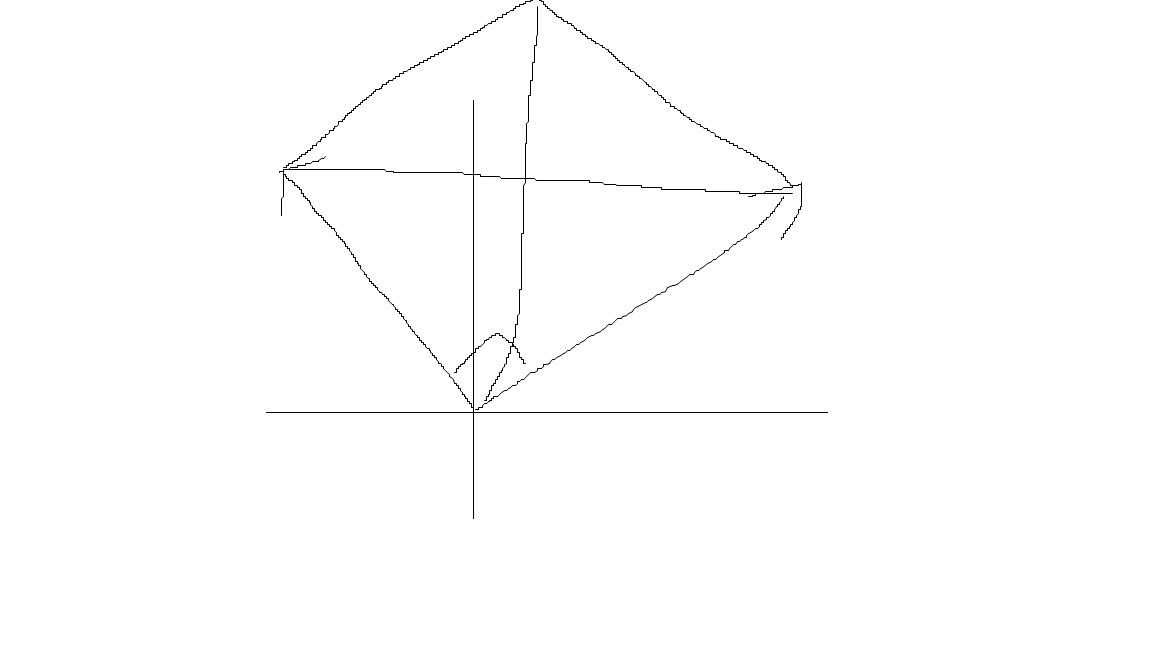
\includegraphics[width=0.7\textwidth]{images/math/1.jpg} %插入图片,[]中设置图片大小,{}中是图片文件名
    % \caption{Main name 2} %最终文档中希望显示的图片标题
    % \label{Fig.main2} %用于文内引用的标签
  \end{figure}
  由于两个向量组成了直角三角形,由勾股定理可知斜边长的平方
  为$v_1^2+v_2^2+w_1^2+w_2^2$. 由于矩形的两个对角线相等,所以该斜边长等于另一个对角
  线的长度. 另一个对角线的终点坐标
  为$(v_1+w_1,v_2+w_2)$,所以$v_1^2+v_2^2+w_1^2+w_2^2=(v_1+w_1)^2+(v_2+w_2)^2$,化简
  即可得$v_1w_1+v_2w_2=0$. $v_1$	
\end{proof}


\newpage
\section{概率论}

\subsection{公理}
\subsection{定义}
\subsection{定理}
\begin{theorem}
样本均值的期望等于总体的期望.
\end{theorem}
\begin{proof}
$x_1,x_2,x_3,...,x_n$与总体X是同分布的,所以各样本的期望均为总体期望。

$E(\bar{X})=E(\frac{1}{n}\sum_{i=1}^{n}x_{i})=\frac{1}{n}\sum_{i=1}^{n}E(x_{i})=\frac{1}{n}\cdot n\cdot E(X)=\mu $
\end{proof}

\begin{theorem}
  $S^2=\frac{1}{n-1}\sum_{i=1}^n(X_i-\overline{X})^2$是样本方差的无偏估计.
\end{theorem}
\begin{proof}
方差无偏估计的推算:

\begin{aligned}
\operatorname{E}[S^{2}]& =\mathrm{E}\left[\frac{1}{n}\sum_{i=1}^{n}\left(X_{i}-\overline{X}\right)^{2}\right]=\mathrm{E}\left[\frac{1}{n}\sum_{i=1}^{n}\left((X_{i}-\mu)-(\overline{X}-\mu)\right)^{2}\right] \\
&=\mathrm{E}\left[\frac{1}{n}\sum_{i=1}^{n}\left((X_{i}-\mu)^{2}-2(\overline{X}-\mu)(X_{i}-\mu)+(\overline{X}-\mu)^{2}\right)\right] \\
&=\mathrm{E}\left[\frac{1}{n}\sum_{i=1}^{n}(X_{i}-\mu)^{2}-\frac{2}{n}(\overline{X}-\mu)\sum_{i=1}^{n}(X_{i}-\mu)+\frac{1}{n}(\overline{X}-\mu)^{2}\sum_{i=1}^{n}1\right] \\
&=\mathrm{E}\left[\frac{1}{n}\sum_{i=1}^{n}(X_{i}-\mu)^{2}-\frac{2}{n}(\overline{X}-\mu)\sum_{i=1}^{n}(X_{i}-\mu)+\frac{1}{n}(\overline{X}-\mu)^{2}\cdot n\right] \\
&=\mathrm{E}\left[\frac{1}{n}\sum_{i=1}^{n}(X_{i}-\mu)^{2}-\frac{2}{n}(\overline{X}-\mu)\sum_{i=1}^{n}(X_{i}-\mu)+(\overline{X}-\mu)^{2}\right] \\
&=\mathrm{E}\left[\frac1n\sum_{i=1}^n(X_i-\mu)^2-\frac2n(\overline{X}-\mu)\cdot n\cdot(\overline{X}-\mu)+(\overline{X}-\mu)^2\right] \\
&=\mathrm{E}\left[\frac{1}{n}\sum_{i=1}^{n}(X_{i}-\mu)^{2}-2(\overline{X}-\mu)^{2}+(\overline{X}-\mu)^{2}\right] \\
&=\operatorname{E}\left[\frac1n\sum_{i=1}^n(X_i-\mu)^2-(\overline{X}-\mu)^2\right] \\
&=\operatorname{E}\left[\frac1n\sum_{i=1}^n(X_i-\mu)^2\right]-\operatorname{E}\left[(\overline{X}-\mu)^2\right] \\
&=\sigma^2-\mathrm{E}\Big[(\overline{X}-\mu)^2\Big]
\end{aligned}

\begin{aligned}
E(\bar{X}-\mu)^2& =E(\bar{X}-E[\bar{X}])^2=var(\bar{X}) \\
&=var\left(\frac{\sum_{i=1}^nX_i}n\right) \\
&=\frac1{n^2}var\left(\sum_{i=1}^nX_i\right) \\
&=\frac1{n^2}\sum_{i=1}^nvar\left(X_i\right) \\
&=\frac{n\sigma^2}{n^2} \\
&=\frac{\sigma^2}n
\end{aligned}

$E[\frac{1}{n}\sum_{i=1}^n(X_i-\overline{X})^2]=\sigma^2-\frac{1}{n}\sigma^2=\frac{n-1}{n}\sigma^2$
\end{proof}

即下式是对方差的无偏估计:

$\mathrm{E}\left[\frac{1}{n-1}\sum_{i=1}^{n}\left(X_{i}-\overline{X}\right)^{2}\right]
=\mathrm{E}\left[\frac{n}{n-1}\frac{1}{n}\sum_{i=1}^{n}\left(X_{i}-\overline{X}\right)^{2}\right]
=\frac{n}{n-1}\frac{n-1}{n}\sigma^2
=\sigma^2$
\end{document}
